\section {Simulation of Previous Works}
\label{simprework}
Since recent years a lot of gait methods on NAO have been developed. Controlling the ZMP is a common technique in gait design. In 2008, Aldebaran Robotics provided in \cite{gouaillier2008nao} an open-loop gait, which is one of the earliest gait methods for the NAO humanoid. The gait is not omni-directional and the maximum speed could only reach approximately \SI{10}{cm/s} according to \cite{graf2009robust}. Moreover, the NAO would not fall down when the ground is flat enough, which means this gait could only provide very poor robustness. Since recent year, some teams in the standard platform league has developed their own gaits, which are outstanding in speed and disturbance rejection. 

In 2009, the team B-Human from University of Bremen already presented a closed-loop gait to increase stability and the maximum speed was \SI{15}{cm/s}. Later in 2010 and 2011, they continuously presented two gaits \cite{Humanoids-Graf-Roefer-10} and \cite{graf2011center} based on 3D inverted pendulum model, whose maximal speed reached \SI{28}{cm/s} and \SI{31}{cm/s} respectively.

In 2014, the team rUNSWift from \ac{UNSW} developed a gait called Walk 2014 which is still popular till nowadays \cite{hengst2014runswift}. The strategy of this gait for next step planning is based on the sensor measurements. As a result, it is quite stable to external disturbances. With the help of this gait, they won the standard platform league competition in 2014 and 2015.

In this section, three gait methods \cite{kajita2003biped, graf2011center, hengst2014runswift} are simulated and compared. Indices of comparison is first introduced in performance evaluation. The algorithm of the three gaits are then described in detailed in the following subsections. Finally, the simulation results are put together and compared. The best gait is found out according to the performance indices.  
\subsection{Performance Evaluation}
In the football competition of robots, a team will be more competitive when its robot players are equipped with a fast and robust gait. Moreover, complex algorithms are time-consuming. Elapse time of running one simulation is also taken into consideration. Performance indices evaluated in this section are: 
\begin{itemize}
	\item Forward walking speed.
	\item CoM swinging offset in $ y $ direction
	\item Ability of disturbance rejection
	\item Elapse time for one simulation
	\item Logical complexity
\end{itemize} 

\subsection{A Zero-Moment Point Previewing Gait}
\label{zmppreviewgait}
The concept of \ac{ZMP} plays a very important role in analysis, synthesis and control of a gait. When the robot is at a single support phase and in equilibrium condition, the forces and moments that acting on the supporting foot should be added to zero. 

The ZMP is defined as the point on ground on which the net moment of the inertial forces and gravity forces has no component along the horizontal axis. When it is lying also inside the foot support polygon, it coincides completely with the \ac{CoP} \cite{vukobratovic2004zero}. However, when the ZMP is outside the support polygon, the ground react force will act on the foot edge, which will cause the robot to rotate about the foot edge and fall over. Planning the ZMP position is one of the most common techniques in robot gait control.

In this part, a gait with preview control scheme proposed in \cite{kajita2003biped} is presented. The robot is modelled by a cart-table, in which the CoM and ZMP position are coupled linearly. The idea of using a preview controller is to use future ZMP positions to generate current ZMP and CoM position. 

\subsubsection{Cart-Table Model}
A cart-table model in the $ y-z $ plane is depicted in Figure {\ref{carttablemodel}}. A cart with mass $ m_c $ is running on a massless table at the height of $ h $ above the ground. The surface of the table free of friction. At the distance of $ d $, the cart possesses velocity $ \dot{d} $ and acceleration $ \ddot{d} $, whose direction depends on on which half of the table the cart is moving. To model the dynamics in $ y $ direction, another set of cart-table model is built in $ x-z $ plane.

\begin{figure}[H]
	\centering
	\includegraphics[width=0.5\linewidth]{fig/carttable.pdf}
	\caption{Cart-table model in $ y-z $ plane}
	\label{carttablemodel}
\end{figure}

It is stated in \cite{kajita2003biped} that, even though the table foot is not wide enough to let the cart stay in table surface, if the cart accelerates properly on the table, the whole system could keep upright for a while, and the ZMP is then inside the table foot polygon at this moment.

The moments should be added up to $ 0 $ around the ZMP according to the its definition: 
\begin{equation}
	m_c\cdot g\cdot(d-p) - m_c\cdot\ddot{d}\cdot h = 0
\end{equation}
which leads to a so-called ZMP equation describing the linear relationship between the positions of ZMP and CoM:
\begin{equation}
p = d-\frac{h}{g}\cdot\ddot{d}.
\end{equation} 



Before it comes to the state-space model, another variable called jerk is introduced, which is the first deviation of acceleration. Taking $ \begin{bmatrix}
d&\dot{d}&\ddot{d}
\end{bmatrix}^T $ as the state vector, the state-space representation of the ZMP equation is written as:

\begin{align}
\label{zmpeuqation}
\begin{split}
\begin{bmatrix}
\dot{d}\\\ddot{d}\\\dddot{d}
\end{bmatrix}
&=
\begin{bmatrix}
0&1&0\\0&0&1\\0&0&0
\end{bmatrix}
\begin{bmatrix}
d\\\dot{d}\\\ddot{d}
\end{bmatrix}+
\begin{bmatrix}
0\\0\\1
\end{bmatrix}\,u\\
p&=
\begin{bmatrix}
1&0&-\frac{h}{g}
\end{bmatrix}
\begin{bmatrix}
d\\\dot{d}\\\ddot{d}
\end{bmatrix}
\end{split}
\end{align}

\subsubsection{Preview Controller}
The ZMP position changes with the switch of the supporting foot, which is a short-lived stage during walking. In other words, the CoM is not able to move synchronously with the ZMP, but has to start taking action before the ZMP changes.

%		\begin{figure}[H]
%			\centering
%			\includegraphics[width=15cm]{fig/zmpref}
%			\caption{ZMP reference trajectories}
%			\label{zmpref}
%		\end{figure}

Therefore, a controller is used in order to preview the ZMP position in the future. In \cite{katayama1985design}, an optimal preview controller is designed for discrete-time systems and is used in ZMP controlling gait 
\cite{kajita2003biped,czarnetzki2009observer,gouaillier2010omni,strom2009omnidirectional}.

The cart-table model in Equation {\ref{zmpeuqation}} is firstly discretized with sampling time $ T_s $ and has the form:
\begin{align}
\label{discretesystem}
\begin{split}
\bm{x}(k+1)&=A\bm{x}(k)+Bu(k),\\
y(k)&=C\bm{x}(k),
\end{split}
\end{align}
where 
\begin{align*}
\begin{split}
\bm{x}(k) &= \begin{bmatrix}
d(kT_s)&\dot{d}(kT_s)&\ddot{d}(kT_s)
\end{bmatrix}^T,\\
u(k)&=u(kT_s),\\
y(k)&=p(kT_s),\\
A&=\begin{bmatrix}
1&T_s&\frac{T_s^2}{2}\\0&1&T_s\\0&0&1
\end{bmatrix},\\
B&=\begin{bmatrix}
\frac{T_s^3}{6}&\frac{T_s^2}{2}&T_s
\end{bmatrix}^T,\\
C&=\begin{bmatrix}
1&0&-\frac{h}{g}
\end{bmatrix}^T.\\
\end{split}
\end{align*}
At each time step $ k $, by defining the differential state vector as $ \Delta\bm{x}(k)=\bm{x}(k) -\bm{x}(k-1)$, the differential control effort as $ \Delta u(k)=u(k)-u(k-1) $ and tracking error as $ e(k)=r(k)-y(k) $, the optimal control law $ u(k) $ previewing $ N  $ time steps in the future is given by: 
\begin{equation}
\label{optimalprecontrol}
u(k)= G_e\sum_{i=0}^{k}e(k)-G_xx(k)-\sum_{l=1}^{N}G_r(l)r(k+l),	
\end{equation}
such that the following performance index is minimized:
\begin{equation}
\label{performanceindex}
J=\sum_{i=k}^{\infty}\left[Q_ee^2(i)+\Delta\bm{x}^T(i)Q_x\Delta\bm{x}(i)+R\Delta u^2(i)\right].
\end{equation}
In Equation {\ref{optimalprecontrol}}, $ G_e $, $ G_x $ and $ G_r $ are gains calculated from the system matrices in Equation {\ref{discretesystem}} and weighted matrices $ Q_e $, $ Q_x $ and $ R $ in Equation {\ref{performanceindex}}. Calculation of these gains is implemented by solving the following discrete-time algebraic Ricatti equation:
\begin{equation}
\tilde{G}_K=\tilde{A}^T\tilde{G}_K\tilde{A}-\tilde{A}^T\tilde{G}_K\tilde{B}\left(R+\tilde{B}^T\tilde{G}_K\tilde{B}\right)^{-1}\tilde{B}^T\tilde{G}_K\tilde{A}+\tilde{Q},
\end{equation}

where 
\begin{align*}
\tilde{B} = \begin{bmatrix}
CB\\B
\end{bmatrix},\,\tilde{F} = \begin{bmatrix}
CA\\A
\end{bmatrix},\,\tilde{I} = \begin{bmatrix}
I\\0
\end{bmatrix},\,\tilde{Q} = \begin{bmatrix}
Q_e&0\\0&Q_x
\end{bmatrix},\,\tilde{A} = \begin{bmatrix}
\tilde{I}&\tilde{F}
\end{bmatrix}.
\end{align*}
And finally the gains are defined as:
\begin{align}
\begin{split}
G_e &= \left(R+\tilde{B}^T\tilde{G}_K\tilde{B}\right)^{-1}\tilde{B}^T\tilde{G}_K\tilde{I},\\
G_x &= \left(R+\tilde{B}^T\tilde{G}_K\tilde{B}\right)^{-1}\tilde{B}^T\tilde{G}_K\tilde{F},\\
G_r(l) &= \left\{\begin{array}{lcl}
-G_e &      & l=1\\
\left(R+\tilde{B}^T\tilde{G}_K\tilde{B}\right)^{-1}\tilde{B}^T\tilde{X}(l-1)     &      & l=2, \cdots, N\\
\end{array}\right. ,
\end{split}
\end{align}

where 
\begin{align*}
\tilde{X}(l)=\left[\tilde{A}-\tilde{B}\left(R+\tilde{B}^T\tilde{G}_K\tilde{B}\right)^{-1}\tilde{B}^T\tilde{G}_K\tilde{A}\right]\tilde{X}(l-1).
\end{align*}


Although the preview controller allows to utilize the future ZMP information to generate current ZMP and CoM positions, it has two limitations as well. Figure {\ref{zmppreviewdrawback}} shows a planned ZMP reference in $ y $ direction within \SI{1}{\second}, together with the ZMP and CoM trajectories output by the cart-table model with this preview controller. The zero position means the ZMP is in the middle between both feet. The ZMP first lies under the left foot (positive ZMP positions) and afterwards under the right foot (negative ZMP positions). Synchronously the torso swings in the same direction and finally back to the upright stance.
\begin{figure}[H]
	\centering
	\includegraphics[width=\linewidth]{fig/ZMPpreviewdrawback.eps}
	\caption[Limitations of the preview controller]{The ZMP reference, ZMP and CoM trajectories in $ y $  direction output from the cart-table model. The preview controller are tuned with parameter $ Q_e = 50500$, $ Q_x =0$, $ R=0.59 $ and $ N=50 $.}.
	\label{zmppreviewdrawback}
\end{figure}

The two limitations can be observed at the start and the end of these trajectories. On one hand, at the beginning, the CoM takes action later than the ZMP reference, which is paradoxical to the idea of using a preview controller. On the other hand, the CoM and the ZMP trajectories are not able to be back to the zero position as the reference does at the end. The reason behind lies in the preview controller. The control effort remains unchanged once the right edge of the preview horizon reaches that of the time horizon. 

To overcome such limitations, an idea is to reserve some space both at the beginning and the end when planning the ZMP. An example is shown in Figure {\ref{zmppreviewspace}}. Now the ZMP tracks the reference and the CoM moves as desired. However, an disadvantage brought by this idea is that, when the robot follows these trajectories, it spends almost \SI{1}{\second} on bringing the torso back to the upright stance without taking any steps, which lowers the walking speed.

Another strategy adopted for the gait design and simulation in this thesis is to plan ZMP reference which lasts much longer than the simulation time. The robot follows this reference until a new one is planned. 
\begin{figure}[H]
	\centering
	\includegraphics[width=\linewidth]{fig/ZMPpreviewdrawback1.eps}
	\caption[Space is reserved to overcome the limitations of the preview controller]{The ZMP reference, ZMP and CoM trajectories in $ y $  direction output from the cart-table model. Extra space at the beginning and the end is reserved. The parameters are unchanged for the preview controller.}.
	\label{zmppreviewspace}
\end{figure}

\subsubsection{Swinging foot motion}
In order to generate joint angles online by using inverse kinematics methods, so that the ZMP and CoM of the robot can follow the references, motions of the swinging foot have to be determined, such as how high it should be lifted and how far it should move to cover a planed step size. %In other words, the foot lifting motion is the curve of the distance between the foot sole and the ground in $ z $ direction; the foot move motion is that between the ankle joint and the CoM in $ x $ or $ y $ direction. 
In this section, the swinging foot motion is generated by first designing some points in space with respect to time and then connecting them with interpolation method called \ac{PCHIP}. 

%\begin{figure}[H]
%	\centering
%	\includegraphics[width=14cm]{fig/pchipcurve}
%	\caption{An example of swinging motion trajectories of one step using PCHIP interpolation. Maximal lifting distance is \SI{1.5}{cm}; maximal moving distance is \SI{4}{cm}.}
%\end{figure} 


\subsubsection{Simulation}
Figure {\ref{zmppreviewblock}} shows the block diagram of the control system of the ZMP previewing gait. $ r_{\mathrm{ZMP}} $ is the planned ZMP trajectory. The ZMP and CoM trajectories output by the cart-table model are references for the robot. Joint angles are calculated by inverse kinematics using these ZMP and CoM trajectories.
\begin{figure}[H]
	\centering
	\includegraphics[width=\linewidth]{fig/zmpcontrolsystem.pdf}
	\caption{Block diagram of the control system using ZMP preview control}
	\label{zmppreviewblock}
\end{figure}

\subsection{A CoM Observing 3D LIPM Gait}
\label{3dlipmgait}
In \cite{Humanoids-Graf-Roefer-10}, a gait based on the 3D \ac{LIPM} is presented and used in the Robocup competition by the team B-Human from University of Bremen in 2010, which is aimed at completely discarding the double support phase during walking. As a result, that they achieved maximum forward speed \si{28} {m/s} and backward speed \si{17} {m/s}, which is twice as fast as what they presented in \cite{graf2009robust} in Robocup 2009.

\subsubsection{3D Linear Inverted Pendulum Model}
A 3D inverted pendulum is shown in Figure {\ref{3dinvertedpendulum}}, whose pivot is fixed at the coordinate system origin $ O $ and bob can move freely in the $ x-y-z $ space. When it is restrained on a plane at the height of $ h $ above the ground, as stated in \cite{kajita2002realtime}, the position and velocity of the bob on that plane relative to the pivot of an inverted pendulum are described by:
\begin{equation}
\label{3dlipm}
\begin{split}
x(t) &= x_0\cdot\cosh(k_c\cdot t)+\frac{\dot{x}_0\cdot\sinh(k_c\cdot t)}{k_c},\\
\dot{x}(t) &= k_c \cdot x_0\cdot\sinh(k_c \cdot t)+\dot{x}_0\cdot\cosh(k_c\cdot t),\\ 
\end{split}
\end{equation}
where $ k_c = \sqrt{\frac{g}{h}} $ is a constant, and $ x_0 $ and $ \dot{x}_0 $ are the position and velocity of the bob with respect to the pivot at $ t= 0 $.
\begin{figure}[H]
	\centering
	\includegraphics[height=0.3\textheight]{fig/ip3d.pdf}
	\caption{3D inverted pendulum}
	\label{3dinvertedpendulum}
\end{figure}
\subsubsection{Support Foot Switching}
A point in time for altering the support leg is used to control the velocity of the CoM in $ y $ direction as well as shifting the origin of the inverted pendulum along $ x $ axis.

$ t=0 $ is the time to alter the support leg and it is also the time where the $ y $ component of the velocity is 0, i.e. $ \dot{x_0}_y=0 $ in Equation {\ref{3dlipm}}.

A single support phase begins at $ t_b $ and ends at $ t_e $, which satisfy:
\begin{align}
\begin{split}
t_b &< 0\\
t_e &> 0\\
\end{split}
\end{align}
which means that the time point $ t=0 $, at which the supporting foot switches, is inside the range between $ t_b $ and $ t_e $. For $ \dot{x}_{0_y}=0 $, the position of the CoM in $ y $ direction can be calculated in time range $ \left[t_b,t_e\right] $ with:
\begin{equation}
x_y(t) = {x_0}_y\cdot\cosh(k_c\cdot t),
\end{equation}
 
Before going on with calculating the time point of foot switching, some coordinate systems on ground about the 3D inverted pendulum have to be defined in advanced.
\begin{figure}[H]
	\centering
	\includegraphics[height=0.3\textheight]{fig/ipy.pdf}
	\caption{Two facing inverted pendulums on the $ y-z $ plane}
	\label{invertedpendulumy}
\end{figure}


Figure {\ref{invertedpendulumy}} shows two facing inverted pendulums depicting the current and next single support phase of the robot, whose CoM is at the height of $ h $ above the ground. $ O $ is the origin of the coordinate system of the current single support phase and $ P $ is the origin of the inverted pendulum, which has a constant distance of $ r_y $ away from $ O $ in a single support phase. At the end of the current single support phase, the distance between the CoM and  the origin is $ x_y(t_e) $. Similarly, for the next single support phase, the origins of the coordinate system and inverted pendulum are denoted as $ \bar{O} $ and $ \bar{P} $ respectively, with a distance of $ \bar{r}_y $. At the starting moment $ \bar{t}_b $, the CoM is at $ \bar{x}_y(\bar{t}_b) $ away from the origin.

Planned step size $ \bar{s}_y $ in $ y $ direction indicates where the robot will place its swinging foot at the end of the current single support phase. When the robot is walking straight, the step size is $ 0 $ and therefore $ \bar{O} $ coincides with $ O $.

\begin{figure}[H]
	\centering
	\includegraphics[height=0.3\textheight]{fig/ipx.pdf}
	\caption[Two facing inverted pendulums on $ x-z $ plane]{Two facing inverted pendulums in $ x-z $ plane. The origins of the inverted pendulum and coordinate system coincide from this perspective of view.}
	\label{invertedpendulumx}
\end{figure}

When the swinging foot is planned to be placed at the location $ \bar{P} $, with a distance of $ \bar{r}_y+\bar{s}_y+r_y $ to $ P $, the following relationships are satisfied:
\begin{align}
\label{facingpendulumy}
\begin{split}
\bar{r}_y+\bar{s}_y+r_y &= \bar{x}_y(\bar{t}_b)+x_y(t_e),\\
\dot{x}_y(t_e)&=\bar{\dot{x}}_y(\bar{t}_b).
\end{split}
\end{align} 

Utilizing the second equations in both Equation {\ref{3dlipm}} and {\ref{facingpendulumy}}, the starting time point of the next single support phase is given by:
\begin{equation}
\bar{t}_b = \frac{1}{k_c}\cdot\asinh\left(\frac{x_{0_y}\cdot\sinh(k_c\cdot t_e)}{{\bar{x}}_0}\right).
\end{equation} 

The problem of finding the end of the current single support phase and the beginning of the next one can be solved iteratively by an end time $ t_e $ being initially guessed. It is updated until the difference between the two sides of the first equation in Equation {\ref{facingpendulumy}} is less than a small constant $ \varepsilon $. This method possesses high computational efficiency: by setting the initial value of $ t_e $ properly, the number of iteration can be suppressed under 10.

\begin{algorithm}[H]  
	\label{computefootswitchtime}
	\caption{Computing the single support duration}
	\begin{algorithmic}[1]
		\STATE  $ t_e \gets$ \text{Initial guess}
		\REPEAT 
		\STATE	$ \bar{t}_b \gets \frac{1}{k_c}\cdot\asinh\left(\frac{{x_0}_y\cdot\sinh(k_c\cdot t_e)}{\bar{x}_{0_y}} \right) $
%		\STATE $ \mathit{temp1} \gets \bar{x}_y(\bar{t}_b)+x_y(t_e)$
		\STATE $ \dot{x}_y(t_e)\gets k\cdot x_{0_y}\cdot\sinh(k_c\cdot t_e) $
		\STATE $ \Delta t_e \gets \frac{\bar{r}_y+\bar{s}_y+r_y-\left(\bar{x}_y(\bar{t}_b)+x_y(t_e)\right)}{2\cdot\dot{x}_y(t_e)} $
		\STATE $ t_e \gets t_e + \Delta t_e $
		\UNTIL $ |\Delta t_e| < \varepsilon$
		\STATE $ \bar{t}_b \gets \frac{1}{k_c}\cdot\asinh\left(\frac{x_{0_y}\cdot\sinh(k_c\cdot t_e)}{\bar{x}_{0_y}}\right) $
	\end{algorithmic}  
\end{algorithm}

So far it has been discussed how to use the dynamics of inverted pendulum on $ y-z $ plane to calculate the time for support foot switching to cover a step size of $ s_y $. As for the dynamics in $ x $ direction, it is stated in \cite{Humanoids-Graf-Roefer-10} and their Code Release \cite{BHumanCodeRelease2010} in 2010 that a distorted pendulum motion equation is adopted:
\begin{equation}
\label{distortedpendulum}
x_x(t)=c_1\cdot\cosh(k_c\cdot t)+c_2\cdot\sinh(k_c\cdot t)+c_3\cdot t + c_4,
\end{equation}
where $ c_1 $, $ c_2 $, $ c_3 $ and $ c_4 $ are parameters that have to be determined to obtain a motion trajectory. The cross section view of the two facing inverted pendulum in $ x-z $ plane is shown in Figure {\ref{invertedpendulumx}}.

Similarly, Equation {\ref{facingpendulumy}} still holds for the motion on $ x-z $ plane when the step size in $ x $ direction is $ s_x $:
\begin{align}
\label{facingpendulumx}
\begin{split}
\bar{r}_x+\bar{s}_x+r_x &= \bar{x}_x(\bar{t}_b)+x_x(t_e),\\
\dot{x}_x(t_e)&=\bar{\dot{x}}_x(\bar{t}_b).
\end{split}
\end{align} 
It is also defined in \cite{Humanoids-Graf-Roefer-10} that the CoM of the inverted pendulum should be directly over its origin at time $ t=0 $ of the next single support phase in $ x $ direction, which leads to $ \bar{x}_{0_x} = 0 $. As a result, the velocity at $ t=0 $ can be calculated by solving Equation {\ref{facingpendulumx}}:
\begin{equation}
\dot{x}_{0_x}=\frac{k_c\cdot\left(\bar{r}_x+\bar{s}_x+r_x\right)}{\sinh(k_c\cdot t_e)+\cosh(k_c\cdot t_e)\cdot\tanh(k_c\cdot\bar{t}_b)},
\end{equation} 
and the parameters $ c_1 $, $ c_2 $, $ c_3 $ and $ c_4 $ in Equation {\ref{distortedpendulum}} can also be determined by combining the following equations:
\begin{align}
\begin{split}
c_1\cdot\cosh(k_c\cdot t_e) + c_2\cdot\frac{1}{k_c}\sinh(k_c\cdot t_e)+c_3\cdot t_e + c_4 &= \bar{s}_x-\bar{x}_x(\bar{t}_b)\\
c_1\cdot k_c\cdot \sinh(k_c\cdot t_e)+c_2\cdot\cosh(k_c\cdot t_e)+c_3 &= \bar{\dot{x}}_x(\bar{t}_b)\\
c_1\cdot\cosh(k_c\cdot t_b) + c_2\cdot\frac{1}{k_c}\sinh(k_c\cdot t_b)+c_3\cdot t_b + c_4 &= x_x(t_b)\\
c_1\cdot k_c\cdot \sinh(k_c\cdot t_b)+c_2\cdot\cosh(k_c\cdot t_b)+c_3 &= \dot{x}_x(t_b)\\			
\end{split}
\end{align}



\subsubsection{Balancing by Observing the CoM}
In \cite{graf2011center}, an different approach of balancing the CoM trajectory is proposed. As soon as a deviation is detected, a new





\subsubsection{Swinging foot motion}
As mentioned in the previous chapter, motions such as foot lifting and moving forwards or sidewards have to be designed for the swinging foot otherwise it is impossible to use inverse kinematics to calculate the joint angles through the gait. As a continuation of their preceding gait methods, this closed-loop 3D LIPM gait utilizes the foot motion presented in \cite{graf2009robust} and \cite{BHumanCodeRelease2009}.
Each step is defined as a phase $ \phi\in\left[0,1\right) $, which is seperated into two halves. In the fist half, the swinging foot is lifted and moved to another position on the ground, while later in the second phase this moved distance is subtracted so that the robot is able to perform some position changes in space.

It is not difficult to find trajectories for foot motions since there are a variety of 2D functions in the world of mathematics. However, it is recommended for two reasons in \cite{BHumanCodeRelease2009} to choose trajectories which can be exactly parametrized to cover different extent of a certain motion and whose second derivation should be small to reduce mechanical stress, which refers to parameterizable and smooth curves. Consequently, several parametrized sinusoidal functions are presented in \cite{graf2009robust}:

\begin{equation}
\label{liftequation}
\mathit{Lift} = \left\{\begin{array}{lcl}
\frac{1-\cos(2\pi(2\phi-x_l)/y_l)}{2} &      &\text{if}\; 2\phi\in\left[x_l,x_l+y_l\right]\\
0     &      & \text{otherwise}\\
\end{array}\right.
\end{equation}

\begin{equation}
\label{moveequation}
\mathit{Move} = \left\{\begin{array}{lcl}
\frac{1-\cos(\pi(2\phi-x_m)/y_m)}{2} &      &\text{if}\; 2\phi\in\left[x_m,x_m+y_m\right]\\
1     &      & \text{if}\; 2\phi\in\left[x_m+y_m,1\right]\\
0	& & \text{otherwise}\\
\end{array}\right.	
\end{equation}

In Equation {\ref{liftequation}} and {\ref{moveequation}}, $ x_l $, $ y_l $, $ x_m $ and $ y_m $ are parameters that can change when the swinging foot is lifted and dropped, i.e. how much a single support phase will take up the whole step. It is natural and can be observed from Figure {\ref{liftmovecurve}} that, the $ \mathit{Move} $ distance will reach it maximum at the moment when the swinging foot is just dropped. Another parameters such as $ \mathit{maxLift} $ and $ \mathit{maxMove} $ can be used to decide how high and far the foot should be lifted and moved. All these parameters are determined during the process of step size planning.

\begin{figure}[H]
	\centering
	\includegraphics[width=12cm]{fig/liftmovecurve.jpg}
	\caption{Lifting and moving motion trajectories for the swinging foot}
	\label{liftmovecurve}
\end{figure}

Figure {\ref{liftmovecurve}} shows lifting and moving trajectories for one foot. Those for another foot are identical except for a delay of half step phase.

\subsubsection{Simulation}

\subsection{Walk2014 from UNSW}
\label{walk2014gait}
The gait Walk2014 is developed by the Robocup team from UNSW since 2014, with which the team rUNSWift won the competition of Robocup Standard Platform League continuously in 2014 and 2015. As one of the successful gaits in recent years, it has been adopted and reformed by another well-performing team B-Human from University of Bremen since 2017\cite{BHumanCodeRelease2017}.

In the team report of UNSW\cite{ratter2010runswift} in 2010, a Fast Walk, whose swinging motion is pendulum-like, is already presented. However, only \SI{80}{\percent} of the time for the foot lifting was used for placing the foot in order to guarantee that the robot will not move a foot that is still treading on ground. In other words, there will be  still \SI{20}{\percent} of double support phase. As a continuation, the Walk2014 aims at eliminating these double support phases.

In this subsection, the Walk2014 integrated with feedback control in both $ x $ and $ y $ direction is simulated and discussed. 

\subsubsection{Inverted Pendulum Dynamics}
Like most of the other gait methods, dynamics in Walk2014 are also first separated in lateral and longitudinal plane and then combined during the implementation. Therefore, since the walking of pendulum-like, the dynamics of the inverted pendulum are first analyzed in both lateral and longitudinal plane.

\begin{figure}[H]
	\centering
	\includegraphics[width=0.7\linewidth]{fig/walk2014pendulumy.pdf}
	\caption{Swinging of robot as well as the inverted pendulum in $ y-z $ plane}
	\label{walk2014lateral}
\end{figure}
Figure {\ref{walk2014lateral}} shows the swinging of the robot from left to right in the lateral plane, which can be modeled by an inverted pendulum, whose bob is depicted in red and coincides with the CoM of the robot. Different from many other gaits in which the foot is parallel to the ground, the ankle roll movement in Walk2014 is canceled so that the foot keeps perpendicular to the leg. Therefore, from this perspective of view, there are four contact points between the feet and the ground, namely the inside and outside edges of each foot. Hence, one of these contact edges is also regarded as the pivot of the inverted pendulum depending on which edge is supporting the whole mass.

\begin{figure}[H]
	\centering
	\includegraphics[width=0.32\linewidth]{fig/walk2014pendulumx.pdf}
	\caption{Swinging of robot as well as the inverted pendulum in $ x-z $ plane}
	\label{walk2014longitudinal}
\end{figure}
Figure {\ref{walk2014longitudinal}} presents the motion of the robot in the longitudinal plane. Similar to the dynamics in the lateral plane, the pivot of the inverted pendulum is at either the front or rear edge of the supporting foot. The swinging foot is tilted so that it it parallel to the ground surface.

\subsubsection{Feedback Control}
In Subsection {\ref{zmppreviewgait}}, the robot is modeled as a cart-table, with which the CoM and ZMP positions are coupled. Future ZMP information can be used to calculate the current ZMP and CoM position. ZMP trajectories are planned for one or several steps before the robot moves. Joint angles are calculated so that the CoM and ZMP trajectories of the robot follow those coming out of the preview controller.  In Subsection {\ref{3dlipmgait}} the dynamic model of the robot is a 3D linear inverted pendulum. In order to eliminate the so-called double support phase, finding the point in time to switch the swinging foot and support foot using Equation {\ref{3dlipm}} is considered. Such methods are called model based.

It is discussed that the dynamics of Walk2014 is pendulum-like, it is not model based but measurement based\cite{BHumanCodeRelease2017}, compared to most of other gaits. The weight, as well as the foot pressure, switches from side to side when the robot is swinging in lateral plane. A single support phase ends when the pressure switching is detected by the sensors equipped under the foot. A next single support phase starts afterwards immediately. As a result, the gait is robust against external disturbances.

In the longitudinal plane, the robot is tilting from back to front during walking. In the report\cite{hengst2014runswift}, a simple but effective way of balancing is proposed: the reading of the pitch gyroscope is passed through a P controller and added the the ankle pitch movement. Therefore, the faster the torso is moving forward, the more pressure the support foot will exert on the ground. The block diagram of such an approach is shown in Figure {\ref{walk2014feedbacklong}}.

\begin{figure}[H]
	\centering
	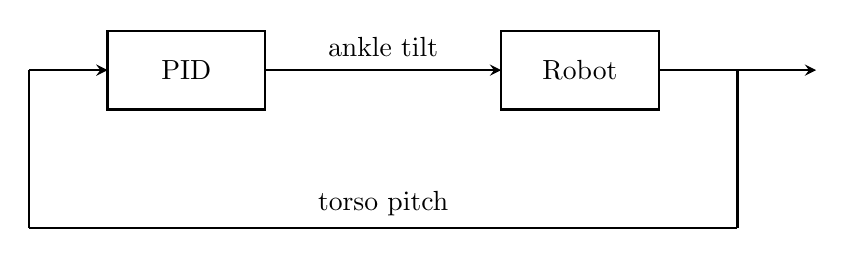
\begin{tikzpicture}
	\draw [black,thick,->,>=stealth] (0,0) -- (1,0);
	
	\draw [black,thick] (1,-0.5) rectangle (3,0.5);
	\draw [black,thick,->,>=stealth] (3,0) -- (6,0);
	\draw [black,thick] (6,-0.5) rectangle (8,0.5);
	\draw [black,thick,->,>=stealth] (8,0) -- (10,0);
	\draw [black,thick] (0,-2) -- (0,0);
	\draw [black,thick] (0,-2) -- (9,-2);
	\draw [black,thick] (9,0) -- (9,-2);
	
	\node at (2,0) {\text{PID}};
	\node at (7,0) {\text{Robot}};
	\node at (4.5,-1.7) {\text{torso pitch}};
	\node at (4.5,0.3) {\text{ankle tilt}};
	\end{tikzpicture}
	\caption{Feedback control of torso tilting on the longitudinal plane}
	\label{walk2014feedbacklong}
\end{figure}

\subsubsection{Simulation}
Since Walk2014 is measurement based, the robot is modelled and controlled by a finite state machine whose states are event triggered, as shown in Figure {\ref{walk2014finitestatemachine}}. Two states $ R $ and $ L $ are responsible for the motion of right and left foot respectively and execute in turn . The state of one foot (e.g. the right foot) is activated when the pressure of another (e.g. the left foot) is greater than a certain value $ P^{*} $. Planning of foot motion includes determining height of lifting, step size and step duration.

\begin{figure}[H]
	\centering
	\includegraphics[width=9cm]{fig/walk2014FSM.pdf}
	\caption{Finite state machine of Walk2014}
	\label{walk2014finitestatemachine}
\end{figure}


As a measurement-based gait, the key of Walk2014 is to have clear and smooth foot pressure measurements. Directly measured foot pressure suffers from strong oscillation, which affects the judgement that whether the foot is completely lifted or dropped. A simple first-order low-pass filter is introduced to the foot pressure measurements:
\begin{equation}
G(s)=\frac{\omega_c}{1+\omega_c},
\end{equation} 
where $ \omega_c $ is the cut-off frequency. The filtered and unfiltered foot pressure are shown together in Figure {\ref{footpressurefilter}}. 
\begin{figure}[H]
	\centering
	\includegraphics[width=\linewidth]{fig/footpressurefilter.eps}
	\caption[Unfiltered and filtered foot pressure within a single support phase]{Unfiltered and filtered foot pressure within a single support phase of \SI{1}{\second}}
	\label{footpressurefilter}
\end{figure}


\subsection{Simulation Results and Comparison}
In this part, the three gaits introduced and simulated in this section are compared from different perspectives according to the indices mentioned in performance evaluation. The best one is chosen as the model for the following sections.

\subsubsection{Walking Speed}
First of all, the walking speeds under a disturbance-free environment are compared. The average speed is calculated by measuring how far the CoM of the robot can move along $ x $ direction within \SI{10}{\second}. The CoM trajectories are shown in Figure {\ref{speedcomparefigure}} and the average speeds are listed in Table {\ref{speedcomparetable}}.

\begin{figure}[H]
	\centering
	\includegraphics[width=\linewidth]{fig/speedcompare.eps}
	\caption{CoM trajectories of three gaits in $ x $ direction with \SI{10}{\second}}
	\label{speedcomparefigure}
\end{figure}

What is noticeable in the figure is that the ZMP previewing gait spends about \SI{2}{\second} on planning the ZMP and CoM trajectories without taking any other motion. The reason is that the strategy of planning ZMP and CoM trajectories lasting much longer than the simulation time. Additionally, Walk2014 is slightly faster than the 3D LIPM gait.
\begin{table}[H]
	\centering
	\caption{Average walking speed of three gaits}
	\label{speedcomparetable}
	\begin{tabular}{ccc}
		\hline
		\text{Gait}&&\text{Speed [\si{cm/s}]}\\
		\hline
		\text{ZMP Previewing Gait}&&\SI{28.11}{cm/s}\\
		\hline
		\text{CoM Observing 3D LIPM Gait}&&\SI{34.07}{cm/s}\\
		\hline
		\text{Walk2014}&&\SI{35.68}{cm/s}\\
		\hline
	\end{tabular}
\end{table}

\subsubsection{Ability of Disturbance Rejection}
\subsubsection{CoM Offset}
CoM offset of straight walking 

ZMP: 0.007

LIPM: 0.006;

Walk2014: arbitrary
\subsubsection{Elapse Time}
In this part, the elapse time for simulating these three methods are compared. The simulation time is \SI{10}{\second} under disturbance-free condition. The result is shown in Table {\ref{elapsetime3method}}. 

\begin{table}[H]
	\centering
	\caption{Elapse time for simulating different gaits}
	\label{elapsetime3method}
	\begin{tabular}{ccc}
		\hline
		\text{Gait}&&\text{Time [s]}\\
		\hline
		\text{ZMP Previewing Gait}&&\SI{84.29}{\second}\\
		\hline
		\text{CoM Observing 3D LIPM Gait}&&\SI{59.84}{\second}\\
		\hline
		\text{Walk2014}&&\SI{49.52}{\second}\\
		\hline
	\end{tabular}
\end{table}

\subsubsection{Logical Complexity}
Since it is not model-based, Walk2014 has the lowest logical complexity among these three gaits. It is easy to be programmed and realized by properly setting condition for support foot switching. The programmed robot has high freedom during steps planning rather than that it has to following some trajectories obtain from the cart-table or inverted pendulum model. However, in real life, the execution of Walk2014 depends highly on the foot pressure sensors. Failure of sensors can lead to incorrect step planning and execution.

\subsection{Conclusion}